\documentclass[11pt]{beamer}
\usepackage[utf8]{inputenc}
\usepackage[T1,T2A]{fontenc}
\usepackage[russian]{babel}
\usepackage{color}
\usepackage{calc}
\usepackage{graphicx}
\usepackage{epstopdf}
\usepackage{hyperref}
\hypersetup{unicode,colorlinks}
\usetheme[progressbar=head,numbering=fraction,block=fill]{metropolis}
\usepackage{minted}
\usepackage{dejavu}
%\usepackage{adjustbox}  % Позволяет сузить куски кода (или текст) ровно настолько, чтобы уместиться в слайд
\usepackage{csquotes}
\usepackage{upquote}

\usemintedstyle{solarized-light}
\newminted[haskell]{haskell}{
    escapeinside=!!,
    mathescape=true,
    texcomments=true,
    beameroverlays=true,
    autogobble=true,
    fontsize=\small,
    breaklines=false  % Лучше сам поставлю переносы на удобных местах
}
\newminted[haskellsmall]{haskell}{
    escapeinside=!!,
    mathescape=true,
    texcomments=true,
    beameroverlays=true,
    autogobble=true,
    fontsize=\footnotesize,
    breaklines=false
}
\newminted[haskelltiny]{haskell}{
    escapeinside=!!,
    mathescape=true,
    texcomments=true,
    beameroverlays=true,
    autogobble=true,
    fontsize=\scriptsize,
    breaklines=false
}
\newmintinline[haskinline]{haskell}{
    escapeinside=!!,
    mathescape=true,
    beameroverlays=true,
    breaklines=true
}
\newminted[ghci]{text}{
    autogobble=true,
    fontsize=\small,
    breaklines=false
}
\newminted[ghcismall]{text}{
    autogobble=true,
    fontsize=\footnotesize,
    breaklines=false
}
\newminted[ghcitiny]{text}{
    autogobble=true,
    fontsize=\scriptsize,
    breaklines=false
}
\newmintinline[ghcinline]{text}{
    breaklines=true
}

\newcommand{\hackage}[1]{\href{https://hackage.haskell.org/package/#1}{#1}}

\vfuzz=20pt  % позволяет тексту дойти до номера слайда

\author{Алексей Романов}
\subtitle{Функциональное программирование на Haskell}
%\logo{}
\institute{МИЭТ}
\subject{Функциональное программирование на Haskell}
%\setbeamercovered{transparent}
%\setbeamertemplate{navigation symbols}{}

\usepackage{syntax}

\title{Лекция 9: функторы, монады и все-все-все}

\begin{document}
    \begin{frame}[plain]
    \maketitle
\end{frame}

\begin{frame}[fragile]
\frametitle{Роды типов}
\begin{itemize}
    \item У значений есть типы, а у типов "--- р\'{о}ды (kinds).
    \item Все обычные типы (\lstinline|Int|, \lstinline|Maybe Bool|, \lstinline|(Int, Int)|, \ldots) имеют род \lstinline|*| (синоним "--- \lstinline|Type|).
    \pause
    \item Пример более сложного рода "--- \lstinline|Maybe|. Он принимает тип рода \lstinline|*| и возвращает тип рода \lstinline|*|: 
    \begin{lstlisting}
    Prelude> :kind Maybe !\pause!
    Maybe :: * -> *
    \end{lstlisting}
    \pause
    \item Определите род: 
    \begin{itemize}
        \item \lstinline!Either! (\lstinline!data Either a b = Left a | Right b!)
        \pause
        \item \lstinline!Shape! (\lstinline|type Shape f = f ()|)
        \pause
    \end{itemize}
    \item В стандартном Haskell все роды строятся из  \lstinline|*| и \lstinline|->|, в GHC всё сложнее (\href{https://downloads.haskell.org/~ghc/8.6.3/docs/html/users_guide/glasgow_exts.html#kind-polymorphism}{Kind polymorphism}, \href{https://downloads.haskell.org/~ghc/8.6.3/docs/html/users_guide/glasgow_exts.html#unboxed-types-and-primitive-operations}{Unboxed type kinds}, \href{https://downloads.haskell.org/~ghc/8.6.3/docs/html/users_guide/glasgow_exts.html#datatype-promotion}{Datatype promotion},  \href{https://downloads.haskell.org/~ghc/8.6.3/docs/html/users_guide/glasgow_exts.html#the-constraint-kind}{The \lstinline|Constraint| kind}).
\end{itemize}
\end{frame}

\begin{frame}[fragile]
\frametitle{Частичное применение типов}
\begin{itemize}
    \item Конструкторы типов могут быть частично применены (как функции).
    \item Если \lstinline!Either :: * -> * -> *!, то \lstinline|Either Int|\pause\lstinline| :: * -> *|. \lstinline|Either a| "--- тоже.
    \pause
    \item Типы кортежей, функций и списков можно писать в префиксном виде: \\
    \lstinline|(,) a b|, \lstinline|(->) a b|, \lstinline|[] a|.
    \pause
    \item И применять частично: \lstinline|(->) Int| читается как \enquote{функции из \lstinline|Int|} и имеет род \pause\lstinline|* -> *|.
    \pause
    \item Синонимы типов (как \lstinline|Shape| с прошлого слайда) всегда должны быть применены полностью.
    \pause
    \item Для частичного применения нужен \\
    \lstinline|newtype Shape f = Shape (f ())|.
\end{itemize}
\end{frame}

\begin{frame}[fragile]
\frametitle{Варианты \lstinline|map|}
\begin{itemize}
    \item Сравним типы нескольких функций:
    \item \alt<-4>{\lstinline|map :: (a -> b) -> [a] -> [b]|}{\lstinline|map :: (a -> b) -> [] a -> [] b|}
    \pause
    \item \lstinline|mapMb :: (a -> b) -> Maybe a -> Maybe b -- mapMaybe называется другая функция|
    \pause
    \item \lstinline|mapMap :: (a -> b) -> Map k a -> Map k b -- Data.Map.{Lazy/Strict}.map|
    \pause
    \item \alt<+>{\lstinline|mapSnd :: (a -> b) -> (c, a) -> (c, b)|}{\lstinline|mapSnd :: (a -> b) -> (,) c a -> (,) c b|} \pause
    \item Видим, что все они имеют вид \pause \\
    \lstinline|forall a b. (a -> b) -> f a -> f b| для разных \lstinline|f| (\lstinline|f| не под \lstinline|forall|!).
\end{itemize}
\end{frame}

\begin{frame}[fragile]
\frametitle{Функторы}
\begin{itemize}
    \item Можем обобщить все функции с предыдущего слайда, введя класс типов
\begin{lstlisting}
class Functor f where
  fmap :: (a -> b) -> f a -> f b
  (<$) :: a        -> f b -> f a
  (<$) = fmap . const
\end{lstlisting}
    \item Здесь \lstinline|f| "--- переменная типа сорта \pause \lstinline|* -> *|.
    \item Смысл \lstinline|fmap g xs|: применить функцию \lstinline|g| ко всем значениям типа \lstinline|a| \enquote{внутри} \lstinline|xs|, не меняя структуры.
    \item \lstinline|(<$)| "--- частный случай \lstinline|fmap|, который иногда может быть реализован напрямую.
    \pause
    \item \lstinline|(<$>)| "--- синоним \lstinline|fmap| как оператор.
\end{itemize}
\end{frame}

\begin{frame}[fragile]
\frametitle{Законы функторов}
\begin{itemize}
    \item Что значит \enquote{не меняя структуры}?
    \item Например, рассмотрим случай \lstinline|fmap id|. Чему должно быть равно \lstinline|fmap id xs|? \pause
\begin{lstlisting}
fmap id xs == xs
\end{lstlisting}
    \pause
    \item Этот закон также формулируется как \\ \alt<+>{\lstinline|fmap id == id|}{\lstinline|fmap (id @a) == id @(f a)|}. \pause
    \item Второй закон функторов:
\begin{lstlisting}
fmap (g . h) xs ==!\pause! fmap g (fmap h xs)
\end{lstlisting}
\pause
\begin{lstlisting}
fmap (g . h)    ==!\pause! fmap g . fmap h
\end{lstlisting}
\end{itemize}
\end{frame}

\begin{frame}[fragile]
\frametitle{Примеры функторов}
\begin{itemize}
    \item Очень многие типы (рода \lstinline|* -> *|) являются функторами. Например:
\begin{lstlisting}
instance Functor Maybe where 
  -- fmap :: (a -> b) -> Maybe a -> Maybe b
  fmap f (Just x) =!\pause! Just (f x)
  fmap _ Nothing  =!\pause! Nothing
\end{lstlisting}
    \pause
    \item 
\begin{lstlisting}
instance Functor [] where 
  fmap =!\pause! map
\end{lstlisting}
    \item Не можем определить
\begin{lstlisting}
instance Functor [] where 
  fmap f xs = []
\end{lstlisting}
\pause
Типы сходятся (проверьте!), но законы нарушены.
\end{itemize}
\end{frame}

\begin{frame}[fragile]
\frametitle{Ещё примеры функторов}
\begin{itemize}
    \item Частично применённые кортежи:
\begin{lstlisting}
instance Functor ((,) c) where 
-- fmap :: (a -> b) -> (c, a) -> (c, b)
fmap f (z, x) =!\pause! (z, f x)
\end{lstlisting}
    \pause
    \item
\begin{lstlisting}
data Pair a = Pair a a
instance Functor Pair where 
-- fmap :: (a -> b) -> Pair a -> Pair b
fmap f (Pair x y) =!\pause! Pair (f x) (f y)
\end{lstlisting}
    \pause
    \item Дома (начните с уточнения типа \lstinline|fmap|):
\begin{lstlisting}
instance Functor (Either c) where ...
instance Functor ((->) c) where ...
\end{lstlisting}
\end{itemize}
\end{frame}

\begin{frame}[fragile]
\frametitle{... и нефункторов}
\begin{itemize}
    \item Не все типы можно сделать функторами! Рассмотрим     
\begin{lstlisting}
newtype Pred a = Pred (a -> Bool)
instance Functor Pred where 
-- fmap :: (a -> b) -> Pred a -> Pred b
fmap g (Pred p) =!\pause! Pred (\x -> ???)
\end{lstlisting}
    \pause \lstinline|g :: a -> b| не к чему применить: у нас нет ничего типа \lstinline|a|!
    \pause
    \item Общее правило: \lstinline|instance Functor F| можно определить, если \lstinline|a| не входит в определение \lstinline|F a| слева от нечётного числа \lstinline|->| (\href{https://downloads.haskell.org/~ghc/8.6.3/docs/html/users_guide/glasgow_exts.html#deriving-functor-instances}{объяснение}).
    \pause
    \item По этому правилу, функтор ли ниже?
\begin{lstlisting}
newtype Tricky a = T ((a -> Int) -> a)
\end{lstlisting}
\end{itemize}
\end{frame}

\begin{frame}[fragile]
\frametitle{Доказательство законов для экземпляра \lstinline|Functor|}
\begin{itemize}
    \item Возьмём для примера \lstinline|instance Functor Pair|. Нужно доказать, что для него:
    \item $\forall$ \lstinline|a :: *|, \lstinline|pair :: Pair a|
\begin{lstlisting}
fmap id pair == pair
\end{lstlisting}
    \pause
    \item Шаг 1: \lstinline|pair = Pair x y|, где \lstinline|x, y :: |\pause\lstinline|a|
\begin{lstlisting}
fmap id pair ==
fmap id (Pair x y) == !\pause! -- определение fmap!\pause!
Pair (id x) (id y) == !\pause! -- определение id!\pause!
Pair x y == 
pair
\end{lstlisting}
    \pause
    \item $\forall$ \lstinline|a, b, c :: *|, \lstinline|pair :: Pair a|, \lstinline|h :: a -> b|, \lstinline|g :: b -> c|
\begin{lstlisting}
fmap (g . h) pair == fmap g (fmap h pair)
\end{lstlisting}
\end{itemize}
\end{frame}

\begin{frame}[fragile]
\frametitle{Использование функторов}
\begin{itemize}
    \item Предскажите результаты:
\begin{lstlisting}
(+ 3) <$> Just 1
(+ 3) <$> Nothing
(+ 3) <$> [1, 2, 3]
\end{lstlisting}
\pause \item[] \item
\begin{lstlisting}
void :: Functor f => f a -> f ()
void x = ???

void [1, 2]
\end{lstlisting}

\end{itemize}
\end{frame}

\begin{frame}[fragile]
\frametitle{Чего не могут функторы?}
\begin{itemize}
    \item Удобно считать, что \lstinline|fmap| берёт функцию \lstinline|a -> b| и \enquote{поднимает} её в тип \lstinline|f a -> f b|.
    \item Можно ли с её помощью поднять функцию двух аргументов? Т.е. можно ли реализовать
\begin{lstlisting}
fmap2 :: Functor f => (a -> b -> c) -> f a -> f b -> f c
fmap2 g fx fy = ???
\end{lstlisting}
\pause
\item Нет! Единственное, с чего мы можем начать: \pause \lstinline|fmap g|. Она имеет тип \pause \lstinline|f a -> f (b -> c)|. 
\item Применив к \lstinline|fx| (тип подходит), получим 
\lstinline|fmap g fx :: f (b -> c)|. \pause
\item Но \lstinline|f (b -> c)| и  \lstinline|f b| скомбинировать уже не получится.
\end{itemize}
\end{frame}

\begin{frame}[fragile]
\frametitle{Аппликативные функторы}
\begin{itemize}
    \item Если добавить к функторам метод получения \lstinline|f c| из \lstinline|f (b -> c)| и \lstinline|f b|, и метод поднятия любого значения, получится понятие аппликативного функтора:
\begin{lstlisting}[basicstyle=\ttfamily\small]
class Functor f => Applicative f where
  pure  :: a -> f a
  infixl 4 <*>, *>, <*
  (<*>) :: f (a -> b) -> f a -> f b
  (*>) :: f a -> f b -> f b
  (<*) :: f a -> f b -> f a
\end{lstlisting}
    \item \lstinline|(*>)| и \lstinline|(<*)| имеют определения по умолчанию.
    \item Теперь можно определить 
\begin{lstlisting}[basicstyle=\ttfamily\small]
liftA2 :: Applicative f => (a -> b -> c) -> 
   f a -> f b -> f c
liftA2 g fx fy = ???
\end{lstlisting}
\end{itemize}
\end{frame}

\begin{frame}[fragile]
\frametitle{Законы аппликативных функторов}
\begin{itemize}
    \item У \lstinline|Applicative| 5 законов:
    \item
\begin{lstlisting}
pure id <*> v = v

pure f <*> pure x = pure (f x)

u <*> pure y = pure ($ y) <*> u

u <*> (v <*> w) = pure (.) <*> u <*> v <*> w

fmap g x = pure g <*> x
\end{lstlisting}
\end{itemize}
\end{frame}

\begin{frame}[fragile]
\frametitle{Моноидальные функторы}
\begin{itemize}
    \item Эти законы не очень удобны и их трудно запомнить. Но мы можем использовать другой класс:
    \item
\begin{lstlisting}[basicstyle=\ttfamily\small]
class Functor f => Monoidal f where
  unit :: f ()
  (**) :: f a -> f b -> f (a,b)
\end{lstlisting}
\item Он взаимовыразим с аппликативными функторами (т.е. \lstinline|pure| и \lstinline|(<*>)| выражаются через \lstinline|unit| и \lstinline|(**)| и наоборот).
\item Законы ($\simeq$: с точностью до изоморфизма):
\begin{lstlisting}[ basicstyle=\ttfamily\small]
unit ** v !$\simeq$! v
u ** unit !$\simeq$! u
u ** (v ** w) !$\simeq$! (u ** v) ** w
\end{lstlisting}
\item Упражнение: записать точные их версии
\end{itemize}
\end{frame}

\begin{frame}[fragile]
\frametitle{Примеры аппликативных функторов}
\begin{itemize}
    \item Многие функторы являются аппликативными:
\begin{lstlisting}[basicstyle=\ttfamily\small]
instance Applicative Maybe where 
  -- pure :: a -> Maybe a
  pure =!\pause! Just
  -- (<*>) :: Maybe (a -> b) -> Maybe a -> Maybe b
  Just g <*> Just x  =!\pause! Just (g x)
  _      <*> _       =!\pause! Nothing
\end{lstlisting}
\pause
\item Для списков есть 2 варианта. Стандартный:
\begin{lstlisting}[basicstyle=\ttfamily\small]
instance Applicative [] where 
  -- pure :: a -> [a]
  pure x =!\pause! [x]
  -- (<*>) :: [a -> b] -> [a] -> [b]
  gs <*> xs =!\pause! [g x | g <- gs, x <- xs]
\end{lstlisting}
\end{itemize}
\end{frame}

\begin{frame}[fragile]
\frametitle{Примеры аппликативных функторов}
\begin{itemize}
    \item Второй аппликативный функтор для списков (определён в \lstinline|Control.Applicative|):
\begin{lstlisting}[basicstyle=\ttfamily\small]
newtype ZipList a = ZipList { getZipList :: [a] }
instance Applicative ZipList where 
  (ZipList fs) <*> (ZipList xs) = ZipList (zipWith ($) fs xs)
  pure x = ???
\end{lstlisting}
    \pause
    \item Подсказка: реализация определяется законом
\begin{lstlisting}[basicstyle=\ttfamily\small]
pure id <*> v = v
\end{lstlisting}
    \pause
    \item Ответ: 
\begin{lstlisting}[basicstyle=\ttfamily\small]
pure x = ZipList (repeat x)
\end{lstlisting}
\end{itemize}
\end{frame}

\begin{frame}[fragile]
\frametitle{Пример неаппликативного функтора}
\begin{itemize}
    \item 
\begin{lstlisting}[basicstyle=\ttfamily\small]
instance Applicative ((,) c) where 
  -- pure :: a -> (c, a)
  pure = ???
\end{lstlisting}
    \pause Невозможно определить без ограничений на \lstinline|c|.
    \pause
    \item А какие ограничения нужны? \pause
\begin{lstlisting}[basicstyle=\ttfamily\small]
instance Monoid c => Applicative ((,) c) where
  pure x = (mempty, x)
  (c1, g) <*> (c2, x) =!\pause! (c1 <> c2, g x)
\end{lstlisting}
\end{itemize}
\end{frame}

\begin{frame}[fragile]
\frametitle{Что можно сделать с аппликативными функторами}
\begin{itemize}
    \item Предскажите результаты:
\begin{lstlisting}[basicstyle=\ttfamily\small]
pure (+) <*> [2, 3, 4] <*> pure 4
[(+1), (*2)] <*> [2, 3]
[1, 2] *> [3, 4, 5]
[1, 2] <* [3, 4, 5]
ZipList [1, 2] *> ZipList [3, 4, 5]
\end{lstlisting}
    \pause
    \item Реализуйте
\begin{lstlisting}[basicstyle=\ttfamily\small]
when :: Applicative f => Bool -> f () -> f ()    
sequenceAL :: Applicative f => [f a] -> f [a]
\end{lstlisting}
    \item У второй есть обобщённая версия \href{http://hackage.haskell.org/package/base-4.12.0.0/docs/Data-Traversable.html#v:sequenceA}{\lstinline|sequenceA|}, определяющая ещё один класс \lstinline|Traversable|.
\end{itemize}
\end{frame}

\begin{frame}[fragile]
\frametitle{... и что нельзя}
\begin{itemize}
    \item Структура результата аппликативного вычисления зависит только от структуры аргументов, а не от значений внутри них. 
    \item Т.е. мы не можем определить функцию
\begin{lstlisting}[basicstyle=\ttfamily\small]
ifA :: Applicative f => f Bool -> f a -> f a -> f a
\end{lstlisting}
так, чтобы выполнялось
\begin{lstlisting}[basicstyle=\ttfamily\small]
ifA [True]  [1, 2] [3] == [1, 2]
ifA [False] [1, 2] [3] == [3]
\end{lstlisting}
(в случае списков структура "--- число элементов).
    \pause
    \item Попробуйте написать какие-нибудь варианты \lstinline|ifA| по типу и убедиться в этом.
    \pause
    \item Эту проблему решают монады, о которых будет следующая лекция.
\end{itemize}
\end{frame}

\begin{frame}[fragile]
\frametitle{Диаграмма классов типов высших родов}
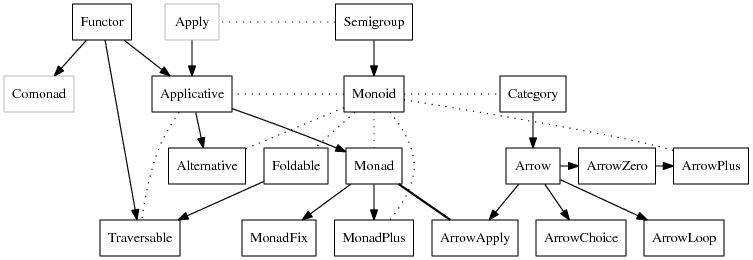
\includegraphics[width=\linewidth]{Typeclassopedia-diagram.png}
\end{frame}

%\begin{frame}[fragile]
%\frametitle{\lstinline|Foldable| и \lstinline|Traversable|}
%\begin{itemize}
%    \item TODO
%\end{itemize}
%\end{frame}
%
%\begin{frame}[fragile]
%\frametitle{Вывод \lstinline|Functor|, \lstinline|Foldable|, \lstinline|Traversable|}
%\begin{itemize}
%    \item TODO
%\end{itemize}
%\end{frame}
%
%\begin{frame}[fragile]
%\frametitle{Монады}
%\begin{itemize}
%    \item TODO
%\end{itemize}
%\end{frame}

\begin{frame}[fragile]
\frametitle{Дополнительное чтение}
\begin{itemize}
    \item \href{https://wiki.haskell.org/Typeclassopedia}{Typeclassopedia} (диаграмма на предыдущем слайде оттуда). Особенно посмотрите на \lstinline|Foldable|, \lstinline|Traversable| и \lstinline|Alternative|.
    \item \href{https://stackoverflow.com/questions/7220436/good-examples-of-not-a-functor-functor-applicative-monad}{Good examples of Not a Functor/Applicative/Monad?}
    \item     \href{http://adit.io/posts/2013-04-17-functors,_applicatives,_and_monads_in_pictures.html}{Functors, Applicatives, And Monads In Pictures.}
    \item Глава \href{https://en.wikibooks.org/wiki/Haskell/Applicative_functors}{Applicative Functors} в Wikibook.
    \end{itemize}
\end{frame}

\end{document}
